\documentclass[border=0.2cm]{standalone}

\usepackage{tikz}
\begin{document}
\pagestyle{empty}
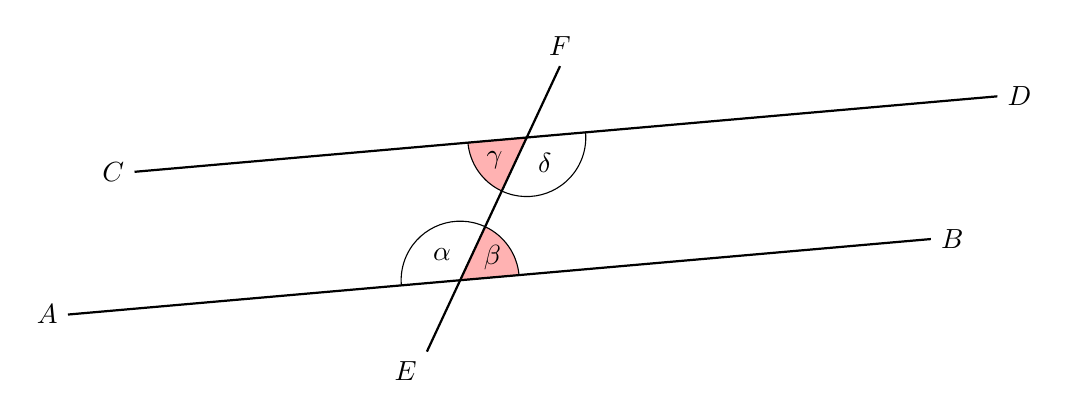
\begin{tikzpicture}[rotate=5]
  \draw (0,0) -- (60:.75cm) arc (60:180:.75cm);
  \draw(120:0.4cm) node {$\alpha$};

  \draw[fill=red!30] (0,0) -- (right:.75cm) arc (0:60:.75cm);
  \draw(30:0.5cm) node {$\beta$};

  \begin{scope}[shift={(60:2cm)}]
    \draw[fill=red!30] (0,0) -- (180:.75cm) arc (180:240:.75cm);
    \draw (30:-0.5cm) node {$\gamma$};

    \draw (0,0) -- (240:.75cm) arc (240:360:.75cm);
    \draw (-60:0.4cm) node {$\delta$};
  \end{scope}

  \begin{scope}[thick]
    \draw (60:-1cm) node[below left] {$E$} -- (60:3cm) node[above] {$F$};
    \draw                   (-5,0) node[left] {$A$} -- (6,0) 
                                        node[right]{$B$};
    \draw[shift={(60:2cm)}] (-5,0) node[left] {$C$} -- (6,0) 
                                        node[right]{$D$};

  \end{scope}
\end{tikzpicture}

\end{document}